\chapter{Experimental Results}
\label{sec:eval}

In this section, we present some preliminary results of the system from five
experiments.  The first two experiments test the precision and recall
of the two main functions, namely title recognition and list extraction,
respectively.
The third one tests the time efficiency and scalability of the whole system.
In the forth experiment, we estimated the total number of ``top-$k$'' pages in the whole web.
And finally, we performed large-scale extraction
on a massive distributed computing platform.
%The first two experiments are done on a PC with 3GB RAM and
%2.7GHz Dual-Core CPU.

\section{Title Recognition}
\label{sec:evalTitle}

We test the performance of the CRF model in this section.
We build a benchmark with 2000 random web page titles,
all of which contains at least one number.
50 of these are ``top-$k$ like'' and are treated as ground truth.

The classifier returns 60 titles, 46 of which are
true positives. Therefore, the precision of the classifier is
$46/60\approx76.7\%$, while the recall is $46/50=92\%$.
The high recall ensures that most of the real ``top-$k$'' pages can pass
through this stage.
The 14 false positives are mostly due to misunderstanding of
some regular phrases, such as ``six pixels of separation''
and ``FIFA 10 cheat codes''.
We can filter these errors in the following stages.




\section{List Extraction}

\label{sec:evalList}

In this section, we test precision and recall of extraction algorithm
which includes the candidate picker and ``top-$k$'' ranker.
%which are realized by the candidate picker and top-$k$ ranker.
The input is the DOM representation of 100 correct ``top-$k$'' pages
as well as the correct title analysis result (number $k$ and concept set).
%As we discussed in Section\ref{sec:picker}, we provide two algorithms:
%{\bf Default} and {\bf +Pattern}.
The result is shown in Table \ref{tab:listRes}.

\begin{table}
\centering
\begin{tabular}{|c||c|c|}
\hline
Algo & Precision & Recall\\\hline
Default & 94.4\% & 85.0\% \\
Def+Patt & 97.4\% & 75.0\% \\
\hline
\end{tabular}
\caption{Results for List Extraction}
\label{tab:listRes}
\end{table}

From this, we can see that both algorithms can obtain very high precision,
while {\em Def+Patt} is slightly higher.
In terms of recall, {\em Default} is better since {\em Def+Patt}
requires stricter patterns.

\section{Time Efficiency}

We also record the average running time for each step to test efficiency,
which is listed in Table \ref{tab:TimeCostDistribution}.
In this table, ``Algo'' means the time cost by the candidate picker and ``top-$k$'' ranker,
``Parse'' is the time for the HTML parser, ``Probase'' is the time cost in Probase Connector, (the number in the bracket is for the MySQL version), and ``Title'' is for the time used by the title classifier.

The data shows high efficiency of our system,
the algorithm only takes up about one fourth of total running time.

In addition, when processing the normal web pages, the system can be even much faster. This is because for most non-``top-$k$'' pages, we can directly filter them without further parsing and analysis, therefore it only takes the Title time to process a normal page,which is less than 10ms.

\begin{table}[tb]
\centering
\caption{Average Execution Time of Different Stages (Unit:ms)}
\label{tab:TimeCostDistribution}
\begin{tabular}{|c||c|c|c|c|}
\hline
\textbf{Total} & Algo & Parse & Probase & Title \\\hline
128 & 33 & 77 & 7(1021) & 9\\\hline

\end{tabular}
\end{table}

Also, we conduct a scaling test of file size,
which is shown in Figure \ref{fig:FileSize}.
The test set are 120 pages with proper size.
The result shows a certain positive correlation between file size and running time.

\begin{figure}[th]
	\centering
	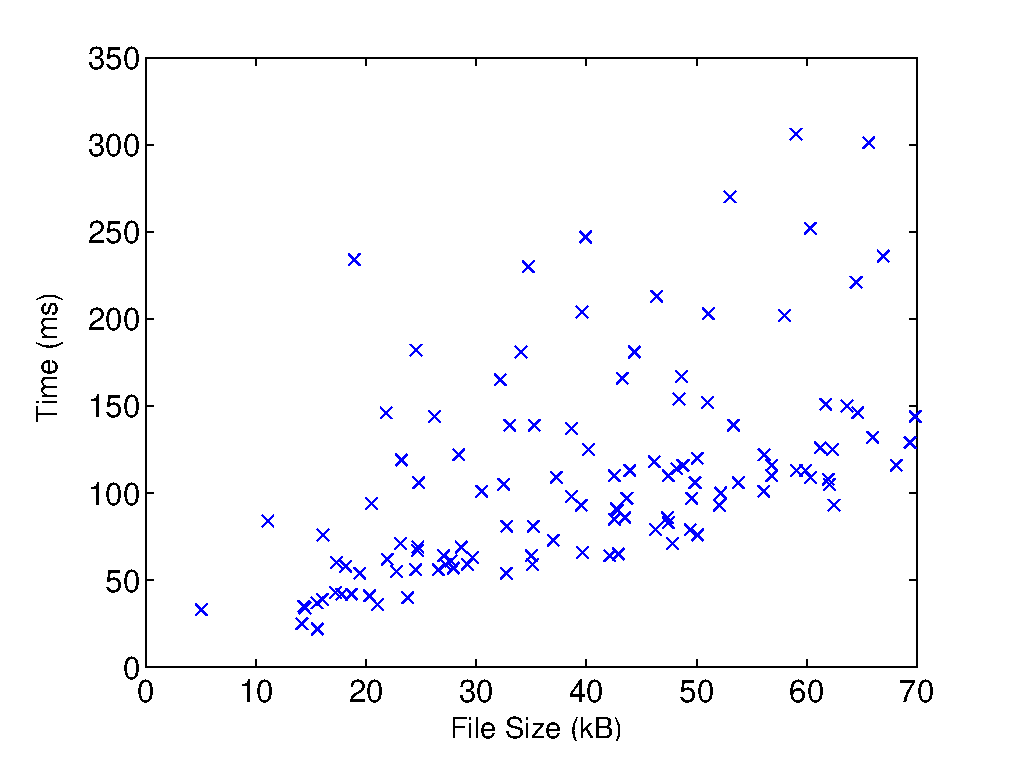
\epsfig{file=./pics/filesize.eps,width=0.9\columnwidth}
	\caption{Scaling Test of File Size}
	\label{fig:FileSize}
\end{figure}



\section{The Sum of Top-K Pages }
\label{sec:topKSum}
As we need to calculate the recall for the overall system, we must estimate the total number of ``top-$k$'' pages.
Known that the recall of the title classifier is 92\%, we use it to identify 1.6 million pages (about 1/1000 of total pages in the web), and obtain 5994 pages.
By manually check these pages, we find 2,061 of them are real ``top-$k$'' pages. Considering there are 8\% missed by the classifier, the total number of ``top-$k$'' pages should be $2,061\div92\%\approx2,240$. Therefore the total number of ``top-$k$'' pages should be approximately $2,240\times1,000=2,240,000$.
Assuming that there are 1.6 billion web pages in total, the proportion of ``top-$k$'' pages are $2,240,000 \div 1,600,000,000\approx0.0014=1.4\textperthousand$.

\section{Big Data}
%One of the purpose for our system is to extract the
%``top-$k$ lists'' from the whole web.
We apply the framework on 1/10 of a high-frequency web snapshot from Bing,
which are about 160 million.
%Since the work of the system is independent,
%the system is easy to run on multiple machines concurrently.
%In this experiment, we apply the system to a distributive computing system to extract data
%To analyze the precision of both algorithm, we randomly sample 100 lists from each result data.
According to the estimated sum of ``top-$k$'' pages,
there should be in total 224,000 ``top-$k$'' pages (ground truth)
in the input data. The detailed result is shown in Table \ref{tab:cosmosRes}.

\begin{table}
\centering
\begin{tabular}{|c||c|c|c|c|}
\hline
Algo & Total & Precision & True Positive & Recall\\\hline
Default & 256,231 & 66.0\% & 169,112 & 75.5\% \\
Def+Patt& 142,886 & 90.4\% & 129,169 & 57.7\% \\
\hline
\end{tabular}
\caption{Results for Big Data}
\label{tab:cosmosRes}
\vspace*{-10pt}
\end{table}

From Table \ref{tab:cosmosRes}, we can see that {\em Def+Patt}
obtains over 90\% precision,
while the recall is lower than {\em Default}. Nevertheless,
{\em Def+Patt} still manage to obtain a large number of ``top-$k$'' lists.
If we project up to the whole web snapshot,
{\em Def+Patt} is expected to get over 1.4 million
``top-$k$ list'' with over 90\% precision.
%
%
%\chapter{Experimental Results}
%\label{sec:eval}
%
%In this section, we present some preliminary results of the system from three
%experiments.  The first two experiments test the precision and recall
%of the two main functions, namely title recognition and list extraction,
%respectively.
%%The third one tests the time efficiency and scalability of the whole system.
%In the last experiment, we performed large-scale extraction
%on a massive distributed computing platform.
%%The first two experiments are done on a PC with 3GB RAM and
%%2.7GHz Dual-Core CPU.
%
%\section{Title Recognition}
%\label{sec:evalTitle}
%
%We test the performance of the CRF model in this section.
%We build a benchmark with 2000 random web page titles,
%all of which contains at least one number.
%50 of these are ``top-$k$ like'' and are treated as ground truth.
%
%The classifier returns 60 titles, 46 of which are
%true positives. Therefore, the precision of the classifier is
%$46/60\approx76.7\%$, while the recall is $46/50=92\%$.
%The high recall ensures that most of the real ``top-$k$'' pages can pass
%through this stage.
%%The 14 false positives are mostly due to misunderstanding of
%%some regular phrases, such as ``six pixels of separation''
%%and ``Fifa 10 cheat codes''.
%%We can filter these errors in the following stages.
%
%\section{List Extraction}
%
%\label{sec:evalList}
%
%In this section, we test precision and recall of extraction algorithm
%which includes the candidate picker and ``top-$k$'' ranker.
%%which are realized by the candidate picker and top-$k$ ranker.
%The input is the DOM representation of 100 correct ``top-$k$'' pages
%as well as the correct title analysis result (number $k$ and concept set).
%%As we discussed in Section\ref{sec:picker}, we provide two algorithms:
%%{\bf Default} and {\bf +Pattern}.
%The result is shown in Table \ref{tab:listRes}.
%
%\begin{table}
%\centering
%\caption{Results for List Extraction}
%\begin{tabular}{|c||c|c|}
%\hline
%Algo & Precision & Recall\\\hline
%Default & 94.4\% & 85.0\% \\
%Def+Patt & 97.4\% & 75.0\% \\
%\hline
%\end{tabular}
%
%\label{tab:listRes}
%\end{table}
%
%From this, we can see that both algorithms can obtain very high precision,
%while {\em Def+Patt} is slightly higher.
%In terms of recall, {\em Default} is better since {\em Def+Patt}
%requires stricter patterns.
%
%\section{Big Data}
%%One of the purpose for our system is to extract the
%%``top-$k$ lists'' from the whole web.
%We apply the framework on 1/10 of a high-frequency web snapshot from Bing,
%which are about 160 million.
%%Since the work of the system is independent,
%%the system is easy to run on multiple machines concurrently.
%%In this experiment, we apply the system to a distributive computing system to extract data
%%To analyze the precision of both algorithm, we randomly sample 100 lists from each result data.
%To calculate the recall, we sampled 10,000 pages from the input data,
%of which 14 are real ``top-$k$'' pages. Therefore,
%we estimate there are in total 224,000 ``top-$k$'' pages (ground truth)
%in the input data. The detailed result is shown in Table \ref{tab:cosmosRes}.
%
%\begin{table}
%\centering
%\caption{Results for Big Data}
%\begin{tabular}{|c||c|c|c|c|}
%\hline
%Algo & Total & Precision & True Positive & Recall\\\hline
%Default & 256,231 & 66.0\% & 169,112 & 75.5\% \\
%Def+Patt& 142,886 & 90.4\% & 129,169 & 57.7\% \\
%\hline
%\end{tabular}
%
%\label{tab:cosmosRes}
%\vspace*{-10pt}
%\end{table}
%
%From Table \ref{tab:cosmosRes}, we can see that {\em Def+Patt}
%obtains over 90\% precision,
%while the recall is lower than {\em Default}. Nevertheless,
%{\em Def+Patt} still manage to obtain a large number of ``top-$k$'' lists.
%If we project up to the whole web snapshot,
%{\em Def+Patt} is expected to get over 1.4 million
%``top-$k$ list'' with over 90\% precision.

